% Generado por `python -m bbfit articulo` (bbfit/articulo.py): no editar a mano; el contenido vive en
% bbfit/articulo.py y es el mismo que la Parte II del PDF docs/articulo/estilos_de_juego_baskonia.pdf.
% Compilar desde docs/articulo/: pdflatex, xelatex o lualatex fit_v2.tex (dos pasadas para el índice); comprobado con tectonic 0.15.
\documentclass[10pt,a4paper]{article}
\usepackage{iftex}
\ifPDFTeX
  \usepackage[utf8]{inputenc}
  \usepackage[T1]{fontenc}
  \usepackage{lmodern}
\else
  \usepackage{fontspec}
\fi
\usepackage[spanish,es-minimal,es-tabla]{babel}
\usepackage{amsmath,amssymb}
\usepackage{booktabs}
\usepackage{graphicx}
\usepackage[margin=2.1cm]{geometry}
\usepackage{xcolor}
\usepackage{caption}
\usepackage{enumitem}
\usepackage[hidelinks]{hyperref}
\setlist{itemsep=2pt,topsep=3pt}
\setlength{\parindent}{0pt}
\setlength{\parskip}{4pt}
\sloppy
\newcommand{\fochopendiente}[1]{\textcolor{red!60!black}{\texttt{[[F8: #1]]}}}
\newenvironment{resumenbox}[1]{\par\medskip\noindent\textbf{#1}\par}{\par\medskip}
\title{Encaje entre ligas (encaje v2): roles, reemplazo, entropía, estilos unificados, adaptación y simulador}
\author{Dirección Deportiva \ensuremath{\cdot} Saski Baskonia --- Modelado y análisis: Claude Code (Anthropic)}
\date{Parte II del artículo «Estilos de juego, roles y encaje entre ligas en quince competiciones de baloncesto»}
\begin{document}
\maketitle
\begin{resumenbox}{Resumen ejecutivo de la Parte II (encaje v2)}
\begin{itemize}
  \item \textbf{Qué añade.} Tres competiciones españolas más (Primera, Segunda y Tercera FEB: 8.102 partidos, 6.369 jugadores) en el mismo esquema que las otras doce, y siete capas de modelo encadenadas: nivel entre ligas con incertidumbre acumulada, rol por minutos y sus cambios, reemplazo de rol, entropía y volatilidad, estilos con la misma definición para jugador y equipo, adaptación al cambio de liga y un simulador de encaje en el que el rol y los minutos son endógenos.
  \item \textbf{Nivel.} El salto hasta la EuroLeague se encadena por un grafo de jugadores puente: Tercera FEB queda a \ensuremath{-}3,46 DT de capacidad EuroLeague con un IC90 de 0,98 (antes 0,41), porque ahora la incertidumbre se suma a lo largo de la cadena. La amortiguación empata con el esquema lineal en error (MAE relativo 1,006 / 1,000) y mejora la cobertura del intervalo del 80 \% (0,829 \ensuremath{\to} 0,841).
  \item \textbf{Rol.} Cinco roles por minutos (RESIDUAL, PROFUNDIDAD, ROTACIÓN, TITULAR, GO-TO-GUY) con un índice de jugador franquicia (GTI): el 93 \% de los diez máximos anotadores de cada liga-temporada sale GO-TO-GUY o TITULAR. Los cambios de rol a mitad de temporada se detectan con un detector bayesiano en línea.
  \item \textbf{Reemplazo.} Un libro contable del volumen de rol por club separa exactamente cuánto de lo que se va se cubre con fichajes, con más minutos de los que ya tenían ese rol o con cambios de rol. La curva uso--eficiencia estimada con variable instrumental tiene signo negativo (rendimientos decrecientes) pero su intervalo incluye el 0.
  \item \textbf{Estilos.} Seis arquetipos con nombre común para jugador y equipo (Spacing, Circulación, Isolation, Old-School, Pistons, Pintura); casi no coinciden con los seis estilos VaDE de la Parte I (ARI 0,031) porque miden otra cosa: la desviación frente a la propia liga, no la vara EuroLeague sin nivel.
  \item \textbf{Adaptación.} Tras la normalización, el estadounidense en su primer año europeo rinde un 6,8 \% [3,8, 9,7] menos de lo esperado que el europeo que cambia de liga; no se adapta más despacio: es un déficit de nivel en esa primera temporada. Corregir la censura (los que no se adaptan dejan de jugar) baja la adaptación media 1-2 puntos.
  \item \textbf{Simulador.} El usuario elige jugador y club; el simulador encadena las capas en ocho pasos Monte Carlo y devuelve minutos, rol, producción con intervalos, un índice Fit descompuesto y avisos. \fochopendiente{resultado principal de la validación del simulador frente a los dos modelos de referencia}
\end{itemize}
\end{resumenbox}
\tableofcontents

\section*{14. Parte II: el sistema de encaje v2}
\addcontentsline{toc}{section}{14. Parte II: el sistema de encaje v2}
La Parte I dice \textbf{cómo juega} un club y sus jugadores, sin el nivel. La Parte II documenta la segunda versión del sistema de encaje, que responde a otra pregunta: \textbf{qué rendimiento, qué rol y qué minutos} cabe esperar de un jugador concreto en un club concreto de otra liga, y con qué incertidumbre. Se construyó en ocho fases, cada una con su código, su configuración YAML (\texttt{configs/\allowbreak{}*.yaml}; el código no fija umbrales), sus pruebas sintéticas, su registro de experimentos en MLflow y un informe de fase (\texttt{docs/\allowbreak{}checkpoints/\allowbreak{}F1.md} \ldots{} \texttt{F8.md}): (F1) ingesta de las competiciones FEB; (F2) normalización con amortiguación del salto de nivel; (F3) sistema de roles por minutos y cambios de rol; (F4) reemplazo de rol; (F5) entropía y volatilidad; (F6) taxonomía unificada de estilos jugador \ensuremath{\leftrightarrow} equipo; (F7) adaptación al cambio de liga; (F8) simulador de encaje.

Todas las formulaciones de esta parte (libro de volumen de rol, descomposición en desplazamiento de minutos y de rol, tasa de relleno, redistribución restringida del uso, asignación endógena de minutos, adaptación y simulador) son propias del proyecto. Todas las cifras proceden de los informes de fase y se citan con su etiqueta: \textbf{[verificado]} = medido en los ficheros de salida; \textbf{[estimado]} = resultado de un modelo, con su intervalo; \textbf{[supuesto]} = hipótesis de trabajo no comprobada del todo. No se ha recalculado ninguna cifra para este documento.

\begin{center}\small
\captionof{table}{Notación común de la Parte II.}
\resizebox{\ifdim\width>\linewidth\linewidth\else\width\fi}{!}{%
\begin{tabular}{ll}
\toprule
Símbolo & Significado \\
\midrule
$i, j$ & jugador; compañero \\
$c = (\ell, t)$ & competición-temporada (liga $\ell$, temporada $t$) \\
$g$ & partido (en la Fase 7: número de partido jugado en la liga nueva) \\
$k$ & rol (Fase 3-4) o estilo (Fase 6) \\
$\theta$ & capacidad latente en desviaciones típicas (DT) de la vara EuroLeague \\
$\delta_c$ & nivel de la competición-temporada $c$ (EuroLeague $=0$ en todas las temporadas) \\
$z,\ z^{*}$ & puesto del jugador en su liga-temporada-posición; $z^{*}$ sin la suerte (paso 1 del algoritmo A) \\
$m_i$ & minutos del jugador por partido del equipo \\
$s_{ik}$ & pertenencia blanda del jugador $i$ al rol $k$ ($\sum_k s_{ik}=1$) \\
$\mathrm{MIN\%}$ & minutos / duración real del partido (con prórrogas; 40' FIBA, 48' NBA y G League) \\
$\mathrm{USG}$, $\mathrm{TS}$ & uso de tiro y acierto real (\%) \\
$L$ & índice de nivel compuesto (8 métricas de nivel, vara EuroLeague) \\
$H$ & entropía en bits \\
$\hat y$ & valor esperado tras la normalización en la escala de la liga de destino \\
\bottomrule
\end{tabular}}
\end{center}

\section*{15. Datos: competiciones FEB (F1)}
\addcontentsline{toc}{section}{15. Datos: competiciones FEB (F1)}
\subsection*{15.1 Alcance, fuente y formatos}
Se añaden tres competiciones españolas al mismo esquema de 480 columnas y a la misma tubería que las doce existentes, sin tablas paralelas: \texttt{feb1} (Primera FEB, antes LEB Oro), \texttt{feb2} (Segunda FEB, antes LEB Plata) y \texttt{feb3} (Tercera FEB, antes Liga EBA). Cada código es una serie histórica: el cambio de nombre de 2024-25 no crea ligas nuevas. Alcance (decisión del usuario): Primera FEB 2022-23 \ensuremath{\to} 2026-27; Segunda y Tercera FEB 2023-24 \ensuremath{\to} 2026-27 (2026-27 en curso). Los grupos (Tercera FEB se juega en 10-31 grupos por temporada; Segunda FEB en Este/Oeste) son un \textbf{atributo del partido}, no una liga.

Fuente pública y anónima de la FEB: calendario por la página de resultados (recorriendo grupos y jornadas con el mismo envío de formulario que hace el navegador), datos de partido de la API JSON que usa la propia web con el «token» de sólo lectura que la página pública entrega a cualquier visitante, y plantillas y entrenador de la página de cada equipo. Cortesía de al menos 1 s entre peticiones por dominio, compartida por todas las ligas del proceso; bruto incremental que nunca se sobrescribe. El jugada a jugada tiene \textbf{dos formatos} [verificado]: estructurado desde 2024-25 (ids y coordenadas de tiro) y sólo texto hasta 2023-24, que se interpreta frase a frase emparejando los nombres abreviados con el boxscore oficial (sin coordenadas). Fases: liga regular = \texttt{regular}; play-offs y fases de ascenso = \texttt{playoffs}; copas y permanencia, fuera.

\begin{center}\small
\captionof{table}{Competiciones FEB ingeridas (informe F1). «Quintetos válidos» = minutos reconstruidos del jugada a jugada a \ensuremath{\leq} 120 s de los oficiales en todos los jugadores del partido; rango por temporada.}
\resizebox{\ifdim\width>\linewidth\linewidth\else\width\fi}{!}{%
\begin{tabular}{llrrrr}
\toprule
Competición (código) & Temporadas & Partidos con datos & Jugadores (id FEB) & Bruto comprimido & Quintetos válidos \\
\midrule
Primera FEB (\texttt{feb1}, antes LEB Oro) & 2022-23 \ensuremath{\to} 2026-27 & 1.295 & 902 & 20 MB & 97,2--99,6 \% \\
Segunda FEB (\texttt{feb2}, antes LEB Plata) & 2023-24 \ensuremath{\to} 2026-27 & 1.216 & 1.147 & 20 MB & 95,1--100 \% \\
Tercera FEB (\texttt{feb3}, antes Liga EBA) & 2023-24 \ensuremath{\to} 2026-27 & 5.591 & 5.151 & 90 MB & 96,2--99,5 \% \\
\bottomrule
\end{tabular}}
\end{center}
\subsection*{15.2 Contrato de datos, posesiones y sesgo de registro}
Un contrato de datos (\texttt{python -m bbstats contrato}) comprueba en cada partido tipos, rangos, identidades ($\mathrm{FGM}=\mathrm{FG2M}+\mathrm{FG3M}$\ldots{}), nulos, clave única partido \ensuremath{\times} equipo \ensuremath{\times} jugador, la suma de minutos del equipo y la coherencia jugada a jugada \ensuremath{\leftrightarrow} boxscore:

\[
\begin{aligned} &\textstyle\sum_{i \in \text{equipo}} \mathrm{min}_{ig} = 200 + 25\,n^{\mathrm{OT}}_{g} \pm 1,\\ &|\mathrm{PTS}^{\mathrm{pbp}} - \mathrm{PTS}^{\mathrm{box}}| = 0,\quad |\mathrm{REB}^{\mathrm{pbp}} - \mathrm{REB}^{\mathrm{box}}| \le 3,\quad |\mathrm{AST}^{\mathrm{pbp}} - \mathrm{AST}^{\mathrm{box}}| \le 2 . \end{aligned}
\]
Resultado [verificado]: 100 \% de los partidos en tipos, rangos, identidades, nulos, clave única y marcador; minutos \ensuremath{\geq} 99 \%; coherencia total desde 2024-25 salvo asistencias de 2024-25 (la fuente a veces no enlaza la asistencia); en 2022-24 (texto) faltan rebotes (coherencia de rebotes del 39-66 \% de los partidos). Las \textbf{posesiones reales} se reconstruyen evento a evento y se comparan con la estimación de caja $P^{\mathrm{box}} = \mathrm{FGA} + 0{,}44\,\mathrm{FTA} - \mathrm{OREB} + \mathrm{TOV}$: la estimación sobrestima en media 0,8 posesiones (\ensuremath{-}1,0 \%) en Primera y 0,7 (\ensuremath{-}0,9 \%) en Segunda y Tercera FEB, con error absoluto medio de 1,6-1,9 posesiones por equipo y partido y correlación 0,89-0,95. \textbf{Sesgo de registro}: las FEB anotan menos asistencias por canasta (0,53-0,54) que el resto de ligas FIBA (0,57-0,66) y un OREB\% algo menor (29,3-29,5 \%); se trata como sesgo de registro al comparar AST\% entre ligas [supuesto].

\subsection*{15.3 Identidad entre ligas}
Una tabla de correspondencia persistente (\texttt{player\_id\_crosswalk.csv}) une los identificadores de las quince ligas en personas por nombre, fecha o año de nacimiento, nacionalidad y calendario, con una confianza en $[0,1]$ y reglas de rechazo (dos fechas de nacimiento completas distintas, años separados más de 1,5, calendario imposible). 23.747 nodos (liga \ensuremath{\times} id) \ensuremath{\to} 16.498 personas; 4.193 en más de una liga; 162 personas FEB unidas automáticamente a otra liga [verificado]. El umbral de fusión pasó de 0,80 a \textbf{0,75} por decisión del usuario (se acepta en bloque la cola de revisión con confianza \ensuremath{\geq} 0,75: 887 uniones nuevas, 11 descartadas por choque de calendario; 39.647 registros, 14.535 personas). Limitaciones: entrenador FEB sólo uno por equipo y temporada (no se ven los relevos); el id FEB de una misma persona cambia a veces; rebotes por quinteto de 2022-24 sesgados a la baja.


\section*{16. Normalización amortiguada del salto de nivel (F2)}
\addcontentsline{toc}{section}{16. Normalización amortiguada del salto de nivel (F2)}
El algoritmo A lleva a cada jugador a la vara EuroLeague con una recta por liga ($a = m_\ell + s_\ell z$). Con las FEB el salto es grande y casi todo indirecto (Tercera \ensuremath{\to} Segunda \ensuremath{\to} Primera \ensuremath{\to} ACB \ensuremath{\to} EuroLeague): una recta única extrapola sin freno y no dice cuánta incertidumbre se acumula. La capa amortiguada (\texttt{bbmodel/\allowbreak{}amortiguacion.py}, \texttt{configs/\allowbreak{}normalization.yaml}) conserva los pasos 1-2 del A (quitar la suerte, $z^{*} = z/(1+v+\psi)$; deriva por edad; escala $s$) y sustituye el nivel de cada competición por seis piezas.

\subsection*{16.1 Encadenamiento jerárquico con acumulación de varianza}
Nodos = competiciones-temporada; aristas = parejas con al menos 3 jugadores puente (\ensuremath{\geq} 150 minutos en las dos, en la misma temporada o al cambiar de liga de $t$ a $t+1$). Cada puente $i$ entre el nodo de menor nivel $x$ y el de mayor nivel $y$ mide el desfase; la arista es su media ponderada con varianza «sándwich», y el nivel de todos los nodos es la solución de mínimos cuadrados ponderados del grafo con la EuroLeague fija en 0:

\[
\begin{aligned} d_i &= g_y(z_y) - g_x(z^{*}_x) - \mathrm{d}(\text{edad})\,\Delta t \;\approx\; \delta_x - \delta_y,\\ \hat\Delta_{xy} &= \frac{\sum_i w_i d_i}{\sum_i w_i}, \qquad V_{xy} = \max\!\big(V^{\mathrm{modelo}}_{xy},\, V^{\mathrm{emp}}_{xy}/n_{xy}\big),\\ \hat{\boldsymbol\delta} &= \arg\min_{\boldsymbol\delta:\ \delta_{\mathrm{EL}}=0} \sum_{(x,y)\in E} \frac{\big(\delta_x - \delta_y - \hat\Delta_{xy}\big)^2}{V_{xy}} . \end{aligned}
\]
En una cadena equivale a \textbf{sumar los desfases y sumar las varianzas}; con dos caminos independientes, a combinarlos por precisión inversa ($V^{-1} = V_1^{-1} + V_2^{-1}$, como resistencias en serie y en paralelo), y lo generaliza a caminos que comparten aristas. El lado $x$ se toma sin suerte ($z^{*}$) y el $y$ tal cual, lo que evita el sesgo de atenuación. Puentes medidos [verificado]: Segunda--Tercera FEB 195, Primera--Segunda 104, ACB--Primera FEB 42, EuroLeague--Primera FEB \textbf{2}, EuroLeague--Segunda o Tercera \textbf{0}.

\subsection*{16.2 Contracción parcial por escalón}
\[
\begin{aligned} \delta_c &\sim \mathcal N\!\big(\mu_{e(c)},\, \tau^2\big), \qquad \mu_e \sim \mathcal N(0,\, 2^2)\ \text{(nodo latente del grafo)},\\ \tau^2 &\leftarrow \tfrac{1}{|C|}\textstyle\sum_c \mathbb E\big[(\delta_c - \mu_{e(c)})^2\big]\ \text{(EM)} , \end{aligned}
\]
con escalones élite (EuroLeague, NBA), doméstica alta (ACB, LBA, BBL, LNB, BSL, GBL), copas europeas (EuroCup, BCL, FEC), desarrollo (G League) y uno por cada FEB. Que $\mu_e$ sea un nodo latente y no una estimación puntual es la diferencia clave: la primera versión daba a Tercera FEB una desviación de 0,06-0,07 tras 4-5 aristas porque trataba la media del escalón como conocida; ahora la incertidumbre común del camino no se reduce por tener cuatro temporadas. Una temporada con pocos puentes (2026-27) se acerca a su escalón.

\subsection*{16.3 Mapeo de cuantiles monótono (probado, no elegido)}
En vez de sólo desplazar, la parte del jugador puede curvarse: $g_\ell(z) = \lambda(d_\ell)\,F_\ell(s_\ell z)$, con $F_\ell$ monótona creciente, $F_\ell(0)=0$ y pendiente 1 fuera de la zona con puentes; se estima por liga y métrica en 7 tramos de cuantiles contraídos hacia la recta con el peso de 30 puentes, regresión isotónica (PAVA) e interpolación monótona PCHIP (ligas con menos de 40 puentes: recta). La variante con mapeo («completo») predijo peor en el examen temporal (MAE relativo 1,0108 y 1,0103 en los cortes 2023 y 2024, frente a 1,0062 y 0,9997 sin mapeo) y \textbf{no se eligió}; queda implementada.

\subsection*{16.4 Transferibilidad \ensuremath{\lambda}(d): estimada \ensuremath{\to} constante}
\[
\begin{aligned} \theta_{\mathrm{ref}} &= \mu_{\mathrm{origen}} + \lambda(d)\,\big(\theta_{\mathrm{trad}} - \mu_{\mathrm{origen}}\big),\\ \lambda(d) &\in \Big\{\,1,\ \ e^{-d/\delta_0},\ \ \frac{1 + e^{-d_0/w}}{1 + e^{(d-d_0)/w}}\,\Big\}, \qquad \lambda \ge 0{,}2 , \end{aligned}
\]
con $\mu_{\mathrm{origen}} = \delta_c$ (el nivel de la competición de origen: lo que se comprime es la distancia del jugador a la media de su propia liga, las colas) y $d_\ell$ = |mediana con signo del desfase en las 8 métricas de nivel| (la mediana y no la media, porque DRtg encadena desfases erráticos). $\hat\lambda$ medida en los puentes = pendiente del valor en destino sobre el traducido con efecto fijo por arista: por encima de 1 en casi todas las ligas (ACB 1,22) y por debajo sólo en Segunda (0,84) y Tercera FEB (0,89), NBA (0,87) y RAPM (\ensuremath{\approx} 0,2-0,4). Error dejando fuera una liga: constante 0,2272, exponencial ($\delta_0 = 30$) 0,2284, logística 0,2509 \ensuremath{\to} \textbf{\ensuremath{\lambda} = 1} [verificado + decisión]. La exponencial (\ensuremath{\lambda} Tercera FEB \ensuremath{\approx} 0,7) sólo gana con el mapeo activo, y esa combinación predice peor.

\subsection*{16.5 Sesgo de selección de los puentes (IPW)}
\[
\begin{aligned} p_i &= \Pr(\text{puente}_i = 1 \mid \text{nivel}_i, \text{nivel}_i^2, \text{edad}_i, \text{edad}_i^2, \log \text{min}_i, \ell, t),\\ w_i &= \operatorname{recorte}_{[p_1,\,p_{99}]}\!\big(1/p_i\big), \qquad w_{\mathrm{puente}} = \sqrt{w_x w_y} . \end{aligned}
\]
Ser puente depende sobre todo de los minutos (+1,08 por log-minuto) y del nivel (+0,30 por DT); los pesos mueven los niveles 0,033 DT de media (0,10 en Tercera FEB, 0,085 en Segunda) [verificado]. Sólo corrige la selección por lo observable (no hay modelo de tipo Heckman).

\subsection*{16.6 Traducción de un jugador, resultados y validación}
\[
\begin{aligned} \theta &= \delta_c + \lambda(d_\ell)\,F_\ell(s_\ell z^{*}), \qquad y_{\mathrm{EL}} = T^{-1}\!\big(\mu_{\mathrm{EL},\mathrm{pos}} + \tau_{\mathrm{EL},\mathrm{pos}}\,\theta\big),\\ \operatorname{Var}(\theta) &= \operatorname{Var}(\delta_c) + (\lambda s F')^2 v_{\mathrm{post}} + (\lambda F)^2 \operatorname{se}(s)^2 . \end{aligned}
\]
\begin{center}\small
\captionof{table}{Nivel por competición antes (A lineal) y después (amortiguado), mediana con signo de las 8 métricas de nivel en DT de capacidad EuroLeague, y anchura del IC90 (informe F2) [verificado].}
\resizebox{\ifdim\width>\linewidth\linewidth\else\width\fi}{!}{%
\begin{tabular}{lrrr}
\toprule
Competición & Antes & Después & IC90 antes \ensuremath{\to} después \\
\midrule
NBA & +0,13 & +0,56 & 0,31 \ensuremath{\to} 0,50 \\
ACB & \ensuremath{-}0,40 & \ensuremath{-}0,23 & 0,19 \ensuremath{\to} 0,26 \\
LNB & \ensuremath{-}0,50 & \ensuremath{-}0,32 & 0,21 \ensuremath{\to} 0,26 \\
BSL & \ensuremath{-}0,77 & \ensuremath{-}0,34 & 0,30 \ensuremath{\to} 0,32 \\
G League & \ensuremath{-}0,52 & \ensuremath{-}0,35 & 0,24 \ensuremath{\to} 0,46 \\
GBL & \ensuremath{-}0,92 & \ensuremath{-}0,41 & 0,28 \ensuremath{\to} 0,34 \\
EuroCup & \ensuremath{-}0,67 & \ensuremath{-}0,42 & 0,19 \ensuremath{\to} 0,27 \\
LBA & \ensuremath{-}0,83 & \ensuremath{-}0,45 & 0,25 \ensuremath{\to} 0,30 \\
BBL & \ensuremath{-}0,91 & \ensuremath{-}0,53 & 0,27 \ensuremath{\to} 0,30 \\
BCL & \ensuremath{-}1,14 & \ensuremath{-}0,57 & 0,35 \ensuremath{\to} 0,31 \\
FEC & \ensuremath{-}1,82 & \ensuremath{-}0,75 & 0,56 \ensuremath{\to} 0,36 \\
Primera FEB & \ensuremath{-}1,02 & \ensuremath{-}1,19 & 0,34 \ensuremath{\to} 0,85 \\
Segunda FEB & \ensuremath{-}1,81 & \ensuremath{-}2,32 & 0,39 \ensuremath{\to} 0,90 \\
Tercera FEB & \ensuremath{-}3,14 & \ensuremath{-}3,46 & 0,41 \ensuremath{\to} 0,98 \\
\bottomrule
\end{tabular}}
\end{center}
\begin{center}
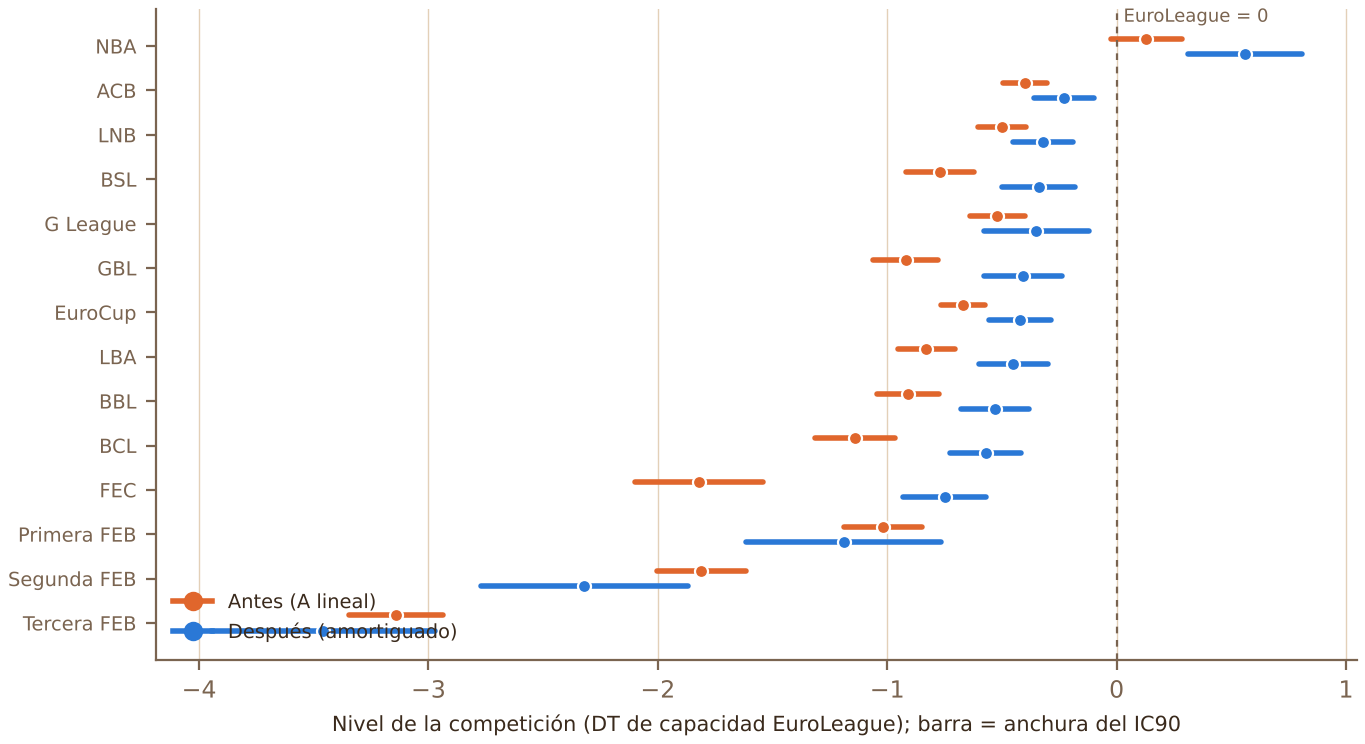
\includegraphics[width=\linewidth]{fit_v2_figuras/fig_ii_niveles.png}
\captionof{figure}{Nivel de cada competición antes y después de la amortiguación (tabla II.3). Las ligas con muchos puentes se acercan a la EuroLeague; las FEB quedan algo más lejos y con intervalos 2-2,5 veces más anchos, porque la incertidumbre se suma a lo largo del camino de puentes.}
\end{center}
\textbf{Validación sin fuga} (ajuste con \ensuremath{\leq} $t$, predicción de $t+1$ de quien cambia de liga con \ensuremath{\geq} 300 min; 722 casos por métrica; la variante se elige con el corte 2023-24 \ensuremath{\to} 2024-25 y se confirma con el 2024-25 \ensuremath{\to} 2025-26). Variante elegida \texttt{sin\_mapeo} (\ensuremath{\lambda} = 1, con IPW): MAE amortiguado / lineal \textbf{1,006 / 1,000}, empate en conjunto; mejor en 13 de 33 métricas (RAPM ofensivo \ensuremath{-}6,5 \%, RAPM \ensuremath{-}3,7 \%, eFG\% \ensuremath{-}2,7 \%, DRtg \ensuremath{-}1,8 \%), peor en pts/100 (+4,4 \%), USG\% (+3,2 \%) y PER (+3,1 \%), sobre todo entre Segunda y Tercera FEB; cobertura del intervalo del 80 \% 0,829 \ensuremath{\to} 0,841. Dejando fuera una liga: si su escalón tiene otras ligas, su nivel se predice con error 0,15 DT (0,32 sin jerarquía) y cobertura del IC90 0,88; en escalones de una sola liga el intervalo es enorme, como corresponde [verificado]. Se corrigió además un fallo de identificación de la varianza de muestreo en la BCL (\ensuremath{\sigma}\ensuremath{^{2}} de pts/100 = $1{,}8\cdot 10^{-4}$ por una recta varianza--exposición con pendiente \ensuremath{\leq} 0): \ensuremath{\sigma}\ensuremath{^{2}} por debajo del 10 \% de la mediana de las otras ligas \ensuremath{\to} esa mediana.


\section*{17. Sistema de roles por minutos y su dinámica (F3)}
\addcontentsline{toc}{section}{17. Sistema de roles por minutos y su dinámica (F3)}
\subsection*{17.1 Tabla partido \ensuremath{\times} jugador}
Para las 15 competiciones y 7 temporadas se reconstruye de los tramos de quinteto y de los tiros una tabla partido \ensuremath{\times} jugador (minutos, titular, minutos del cierre y del 4.º cuarto, posesiones y +/- en pista, tiros propios y del equipo en pista), que incluye las \textbf{ausencias} (partidos del equipo entre el primero y el último del jugador en los que no salió), necesarias para detectar vacíos de rol. Donde una liga-temporada tiene menos del 50 \% de los partidos con tramos se usa la caja (BBL 2020-23, LNB 2020-21, BCL 2020-21; 1.696 de 40.084 registros).

\[
\begin{aligned} \mathrm{MIN\%}_{ig} &= \frac{\mathrm{min}_{ig}}{D_g}, \qquad \bar m_i = 40\cdot\overline{\mathrm{MIN\%}}_i, \qquad \mathrm{USG}_{ig} = 100\,\frac{\mathrm{FGA}_{ig} + 0{,}44\,\mathrm{FTA}_{ig}}{\mathrm{FGA}^{\mathrm{on}}_{g} + 0{,}44\,\mathrm{FTA}^{\mathrm{on}}_{g}},\\ \mathrm{CLOSE}_{ig} &= \sum_{\text{tramos } [a,b]} \big|[a,b] \cap W_g\big|\;\mathbf 1\{|\text{margen}_a| \le 5\}, \end{aligned}
\]
con $D_g$ la duración real del partido (prórrogas incluidas), $W_g$ los últimos 300 s de cada periodo \ensuremath{\geq} 4 y el margen al empezar el tramo. El uso es «de tiro» porque no hay pérdidas por jugador y partido; la versión de caja va al lado [supuesto: el orden por uso cambia poco].

\subsection*{17.2 Reglas de rol y GTI}
\[
\mathrm{rol}_i = \begin{cases} \text{RESIDUAL} & \bar m_i < 5\\ \text{PROFUNDIDAD} & 5 \le \bar m_i < 15\\ \text{ROTACIÓN} & 15 \le \bar m_i < 22, \text{ o } 22 \le \bar m_i < 25 \text{ sin } \mathcal T_i\\ \text{TITULAR} & \bar m_i \ge 25, \text{ o } 22 \le \bar m_i < 25 \text{ con } \mathcal T_i:\ \mathrm{GS\%}_i \ge 0{,}5 \,\lor\, \mathrm{CLOSE\%}_i \ge 0{,}5\\ \text{GO-TO-GUY} & \bar m_i \ge 22,\ \operatorname{rango}_{\mathrm{equipo}}(\mathrm{GTI}_i) \le 2,\ \mathrm{GTI}_i \ge 1{,}0 \cdot \textstyle\sum_c w_c \end{cases}
\]
\[
\begin{aligned} \mathrm{GTI}_i &= \sum_{c} w_c\, z_{ic}, \qquad c \in \{\mathrm{USG},\ \mathrm{PIE},\ \%\,\text{no asistidas},\ \mathrm{USG}^{\mathrm{cl}}\},\ \ w_c = 1,\\ \tilde u^{\mathrm{cl}}_i &= \frac{n^{\mathrm{cl}}_i u^{\mathrm{cl}}_i + 15\,u_i}{n^{\mathrm{cl}}_i + 15}, \qquad \tilde q_i = \frac{\mathrm{FGM}^{\mathrm{na}}_i + 20\,\bar q_\ell}{\mathrm{FGM}_i + 20} . \end{aligned}
\]
Los umbrales se expresan sobre 40' (MIN\% = minutos/40; en NBA y G League el mismo MIN\% equivale a minutos/48 \ensuremath{\cdot} 48). Las $z$ se calculan dentro de la liga-temporada sobre los jugadores con MIN\% \ensuremath{\geq} 25 \% y \ensuremath{\geq} 5 partidos; el USG\% del cierre se contrae hacia el global ($k$ = 15 intentos de equipo) y el \% no asistido hacia la media de la liga ($k$ = 20 canastas). Exigir top-2 del equipo \textbf{y} un umbral absoluto (z medio \ensuremath{\geq} 1) deja \ensuremath{\approx} 1 GO-TO-GUY por equipo; con sólo el top-2 salían \ensuremath{\approx} 2 (en ACB, 27 GO-TO-GUY frente a 23 TITULAR).

\subsection*{17.3 Muestra pequeña: vector de rol}
\[
p_{ik} = \frac{n_{ik} + \alpha\,\pi_{\ell t,k}}{n_i + \alpha}, \quad \alpha = 2, \qquad H^{\mathrm{rol}}_i = -\sum_k p_{ik}\log_2 p_{ik} ,
\]
con $n_{ik}$ los partidos del jugador en el estado $k$ (cada partido recibe un estado con la misma regla) y $\pi$ el reparto de la liga-temporada. Con menos de 5 partidos no hay etiqueta dura (\texttt{rol\_probabilistico}); el vector se calcula para todos y es la pertenencia blanda $s_{ik}$ que usa el reemplazo (F4). Un 28 \% de los registros son probabilísticos (jugadores de paso y la temporada en curso).

\subsection*{17.4 Cambios de rol: detección bayesiana en línea (BOCPD)}
Sobre la serie $x_g = (\mathrm{MIN\%}_g, \mathrm{USG}_g)$ de cada jugador-equipo-temporada se aplica una detección bayesiana en línea de puntos de cambio (implementación propia) con longitud de tramo $r_g$, riesgo constante $H$ y, para cada componente, media desconocida con previa normal y ruido conocido (varianza partido a partido dentro de jugador por liga-temporada, con suelo; las dos series independientes; un partido con menos de 8' no aporta USG):

\[
\begin{aligned} \Pr(r_g = r+1, x_{1:g}) &= \Pr(r_{g-1} = r, x_{1:g-1})\; \pi_r(x_g)\,(1-H),\\ \Pr(r_g = 0, x_{1:g}) &= \textstyle\sum_r \Pr(r_{g-1}=r, x_{1:g-1})\; \pi_r(x_g)\,H, \qquad H = \tfrac{1}{20},\\ \pi_r(x_g) &= \mathcal N\!\big(x_g \mid \mu_r,\ v_r + \sigma^2\big), \quad v_r = \big(v_0^{-1} + r\,\sigma^{-2}\big)^{-1}, \quad \mu_r = v_r\Big(\frac{\mu_0}{v_0} + \frac{1}{\sigma^2}\textstyle\sum_{h=g-r}^{g-1} x_h\Big). \end{aligned}
\]
Un tramo empieza en $s$ si $\Pr(r_{s+4} = 5 \mid x_{1:s+4}) \ge 0{,}5$ (confirmación con 4 partidos posteriores), con tramos de al menos 4 partidos. Un cambio de entrenador abre tramo (los interinos de menos de 3 partidos se funden con el bloque vecino) y un traspaso crea otro registro. Cada cambio lleva covariables: cambio de entrenador en \ensuremath{\pm}4 partidos, \textbf{vacío de rol} (compañero de su posición con MIN\% medio \ensuremath{\geq} 50 \% en los 4 previos que no juega \ensuremath{\geq} 50 \% de los 4 siguientes), fichaje en su posición (compañero que debuta con el equipo en marcha y juega \ensuremath{\geq} 30 \% de los minutos) y rendimiento reciente (TS\% y +/- por 40 de los 4 previos).

\subsection*{17.5 Resultados y validación}
\begin{center}
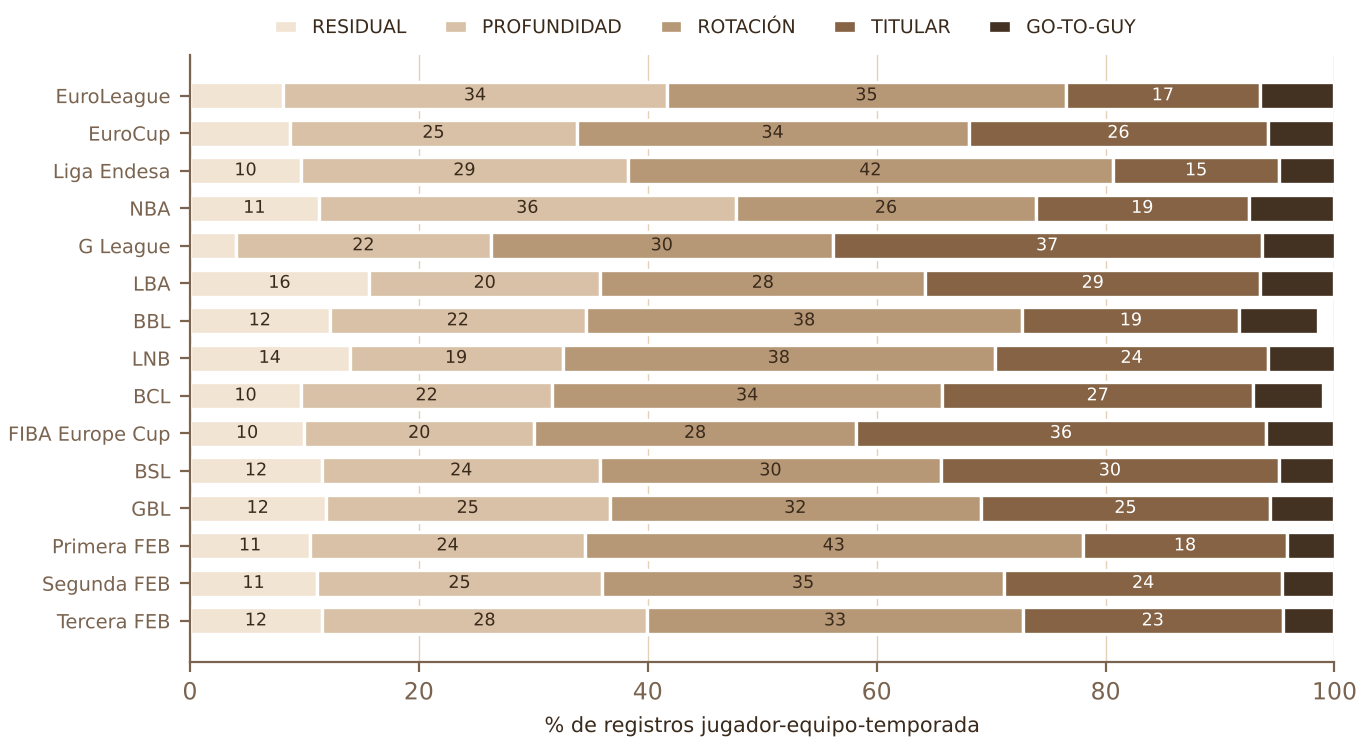
\includegraphics[width=\linewidth]{fit_v2_figuras/fig_ii_roles.png}
\captionof{figure}{Reparto de roles por competición (\% de registros jugador-equipo-temporada; \texttt{distribucion\_roles.csv}). Rol ordinal en una rampa de un solo tono, de RESIDUAL (claro) a GO-TO-GUY (oscuro).}
\end{center}
[verificado] De los diez máximos anotadores de cada liga-temporada, el 60 \% sale GO-TO-GUY y el \textbf{93 \%} GO-TO-GUY o TITULAR (EuroLeague 81 \% GO-TO-GUY; NBA 98 \%); Jokić, Dončić y Gilgeous-Alexander son GO-TO-GUY en las seis temporadas completas; Huertas, en la ACB de 2020-21 a 2025-26; Markus Howard es ROTACIÓN en 2022-23 (19-20' con USG 33-36 \%) y GO-TO-GUY en 2023-24: la regla separa uso de minutos. El 100 \% de los jugadores con menos de 5' y \ensuremath{\geq} 5 partidos es RESIDUAL. Tramos: 1,11 por jugador-equipo-temporada, mediana de 11 partidos; inicios por temporada 36.947, entrenador nuevo 2.597, cambio detectado 1.735, traspaso 1.441. En los cambios detectados [estimado: asociaciones descriptivas] hay vacío de rol en el 28,5 \% (43 \% de las subidas de minutos frente al 12 \% de las bajadas) y fichaje en su posición en el 22 \% (24 \% de las bajadas); antes de una bajada, el TS\% de los 4 partidos previos está 0,46 puntos por debajo de su media previa. Estructura de equipo (mediana por liga): 8-13 jugadores de rotación, HHI de minutos 0,082-0,108 y los dos jugadores de más uso concentran el 27-34 \% del uso.


\section*{18. Reemplazo de rol (F4)}
\addcontentsline{toc}{section}{18. Reemplazo de rol (F4)}
Cuando un club pierde a un jugador no pierde «un nombre», pierde un \textbf{volumen de rol}: minutos ejercidos con una determinada mezcla de roles. Esta sección formaliza cómo se reparte ese volumen (libro contable), cuánto cuesta en eficiencia asumir más uso (elasticidad), cómo se cierra el reparto del uso en la plantilla (suma fija) y cómo se asignan los minutos de forma endógena (\texttt{bbfit/\allowbreak{}reemplazo.py}, \texttt{configs/\allowbreak{}reemplazo.yaml}).

\subsection*{18.1 Libro de volumen de rol y descomposición minutos / rol}
\[
V_k(c,t) = \sum_{i \in (c,t)} m_i\, s_{ik}, \qquad D_k = \sum_{i \in \mathcal S} m_i s_{ik}, \qquad I_k = \sum_{i \in \mathcal A} m'_i s'_{ik},
\]
\[
\begin{aligned} \underbrace{m'_i s'_{ik} - m_i s_{ik}}_{i \in \mathcal C} &= \underbrace{(m'_i - m_i)\,s_{ik}}_{\text{desplazamiento de minutos}} + \underbrace{m'_i\,(s'_{ik} - s_{ik})}_{\text{desplazamiento de rol}},\\ V'_k - V_k &= I_k - D_k + \mathrm{DM}_k + \mathrm{DR}_k, \qquad \mathrm{DM}_k = \textstyle\sum_{\mathcal C}(m'_i - m_i)s_{ik},\ \ \mathrm{DR}_k = \sum_{\mathcal C} m'_i(s'_{ik} - s_{ik}) , \end{aligned}
\]
\[
R_k = \frac{I_k + \mathrm{DM}_k + \mathrm{DR}_k}{D_k} \qquad \text{(tasa de relleno, sin tope)},
\]
con $\mathcal S$ los que se van, $\mathcal A$ los que llegan y $\mathcal C$ los que siguen entre $t$ y $t+1$; $m_i$ son minutos por partido del equipo (así son comparables temporadas con distinto número de partidos) y $s_{ik}$ el vector de rol de la F3. La identidad es \textbf{exacta}: error máximo medido $1{,}0\cdot 10^{-13}$ minutos en 1.332 transiciones club-temporada [verificado]. La estrategia dominante del relleno es el mayor de los tres términos ($I_k$ externa, $\mathrm{DM}_k$ interna por minutos, $\mathrm{DR}_k$ interna por rol). El club estable entre temporadas es el \texttt{team\_id}, salvo en las FEB (código de club: el id de inscripción cambia cada año).

\begin{center}\small
\captionof{table}{Volumen CLAVE (TITULAR + GO-TO-GUY) entre temporadas y su asociación con el cambio de Net del equipo (temporadas cerradas, IC 90 \% bootstrap; asociación, no causalidad) [verificado].}
\resizebox{\ifdim\width>\linewidth\linewidth\else\width\fi}{!}{%
\begin{tabular}{lr}
\toprule
Medida & Valor \\
\midrule
Mediana de salidas / llegadas (minutos por partido) & 55,3' / 52,2' \\
Mediana del desplazamiento de minutos / de rol & \ensuremath{-}1,1' / +0,5' \\
Tasa de relleno $R$ (mediana; p25--p75) & 0,96 (0,72--1,19) \\
Estrategia dominante: externa / interna por rol / interna por minutos & 1.236 / 76 / 16 \\
\ensuremath{\Delta} Net, relleno externo (n = 932) & \ensuremath{-}0,10 [\ensuremath{-}0,45, +0,23] \\
\ensuremath{\Delta} Net, interno por minutos (n = 13) & +3,8 [+2,1, +5,7] \\
\ensuremath{\Delta} Net, interno por rol (n = 70) & \ensuremath{-}3,2 [\ensuremath{-}4,3, \ensuremath{-}2,1] \\
Correlación de rangos relleno \ensuremath{\leftrightarrow} \ensuremath{\Delta} Net & \ensuremath{-}0,08 [\ensuremath{-}0,13, \ensuremath{-}0,03] \\
\bottomrule
\end{tabular}}
\end{center}
Lectura prudente: los clubes que reparten el volumen clave a quienes ya tenían ese rol (más minutos) mejoran; los que lo cubren cambiando de rol a otros empeoran. Puede ser al revés (equipos en crisis reorganizan roles) y $n$ es pequeño en «interna por minutos». \textbf{Transiciones} de los que siguen (3.551 jugadores con \ensuremath{\geq} 300' en ambas temporadas): persistencia GO-TO-GUY 0,68, TITULAR 0,63, ROTACIÓN 0,60, PROFUNDIDAD 0,49; GO-TO-GUY \ensuremath{\to} TITULAR 0,24; PROFUNDIDAD \ensuremath{\to} ROTACIÓN 0,45; movimiento medio del vector de rol (distancia de variación total) 0,27.

\subsection*{18.2 Elasticidad uso--eficiencia con variable instrumental}
La regresión dentro de jugador de TS\% sobre USG\% sale \textbf{positiva} (partido a partido \ensuremath{\beta} \ensuremath{\approx} +0,23 en exteriores, +0,14 en aleros, \ensuremath{-}0,01 en interiores): no son rendimientos crecientes, es \textbf{selección} (el que acierta sigue tirando). Por eso el uso de cada partido se instrumenta con el \textbf{vacío de rol del día}, la cuota de uso de temporada de los compañeros de rotación ausentes, y $\beta$ se agrupa parcialmente por posición:

\[
\begin{aligned} \mathrm{USG}_{ig} &= \pi\, Z_{ig} + \alpha_i + u_{ig}, \qquad Z_{ig} = \sum_{j \in \mathcal R_i,\ j \text{ ausente en } g} \mathrm{cuota\ de\ uso}_j \qquad (\mathcal R_i:\ \mathrm{MIN\%}_j \ge 25\,\%),\\ \mathrm{TS}_{ig} &= \beta\,\widehat{\mathrm{USG}}_{ig} + \alpha_i + e_{ig}, \qquad \beta_i^{*} = w_i\,\hat\beta_i + (1-w_i)\,\beta_g, \qquad w_i = \frac{\tau_g^2}{\tau_g^2 + \mathrm{se}_i^2} , \end{aligned}
\]
con efectos fijos $\alpha_i$ de jugador-equipo-temporada y $\hat\beta_i$ propio sólo si su primera etapa es fuerte ($F_i \ge 10$). Primera etapa: +3,8 puntos de USG\% por cada 100 \% de cuota de uso ausente ($F \approx 1.500$) [estimado]. Supuesto de exclusión: la ausencia sólo afecta al TS\% del jugador a través de su uso [supuesto].

\begin{center}\small
\captionof{table}{Elasticidad uso--eficiencia por variable instrumental (\ensuremath{\Delta}TS\% por +1 punto de USG\%; IC 90 \% por bootstrap de personas) [estimado].}
\resizebox{\ifdim\width>\linewidth\linewidth\else\width\fi}{!}{%
\begin{tabular}{lrlrr}
\toprule
Grupo & \ensuremath{\beta} & IC 90 \% & Filas & Personas \\
\midrule
Exteriores (E) & \ensuremath{-}0,014 & [\ensuremath{-}0,22, +0,20] & 245.889 & 5.409 \\
Aleros (A) & \ensuremath{-}0,170 & [\ensuremath{-}0,58, +0,26] & 77.318 & 1.736 \\
Interiores (I) & \ensuremath{-}0,159 & [\ensuremath{-}0,49, +0,16] & 193.041 & 4.416 \\
Todos & \ensuremath{-}0,076 & [\ensuremath{-}0,22, +0,08] & 517.487 & 12.177 \\
\bottomrule
\end{tabular}}
\end{center}
El signo es negativo (rendimientos decrecientes), pero \textbf{los intervalos incluyen el 0}. Sólo 175 jugadores tienen primera etapa individual fuerte; la heterogeneidad $\tau^2$ queda en el suelo y $\beta_i^{*} \approx \beta_g$ para casi todos: no hay información para distinguir jugadores, y el simulador debe propagar el intervalo, no la media. Pérdidas (entre temporadas, sin instrumento posible): $\gamma \approx -0{,}09$ (E), \ensuremath{-}0,07 (I), +0,04 (A) por punto de USG\%: asociación, no efecto.

\subsection*{18.3 Proyección a un rol y redistribución restringida del uso}
\[
\begin{aligned} \Delta\mathrm{USG} &= \mathrm{USG}_{\mathrm{dest}}(k) - \mathrm{USG}_{\mathrm{orig}}(k), \qquad \mathrm{TS}' = \mathrm{TS} + \beta_i\,\Delta\mathrm{USG},\ \ \beta_i \sim \mathcal N(\beta^{*}_i, \mathrm{sd}_i^2),\\ \mathrm{P100}' &= \mathrm{P100}\cdot\frac{\mathrm{USG}'}{\mathrm{USG}}\cdot\frac{\mathrm{TS}'}{\mathrm{TS}} . \end{aligned}
\]
La producción por 100 no es invariante al rol (EuroLeague, medianas de RESIDUAL a GO-TO-GUY: USG\% 15,0 / 16,4 / 19,3 / 19,7 / 26,8 y puntos por 100 posesiones 11,1 / 17,3 / 22,0 / 22,8 / 30,4; Tercera FEB 9,7 \ensuremath{\to} 26,5) [verificado]: escalar a un jugador de PROFUNDIDAD a GO-TO-GUY con su producción de banquillo mezcla rol y nivel. La plantilla se cierra con dos restricciones de suma fija: las salidas liberan minutos y volumen de uso, las llegadas absorben el suyo y los que siguen se reescalan:

\[
\begin{aligned} &\textstyle\sum_i \mathrm{min}_i = 5\,T, \qquad \sum_i \mathrm{min}_i\,\frac{\mathrm{USG}_i}{100} = T \quad (\text{USG medio en pista } 20\,\%),\\ &\mathrm{min}_i \leftarrow \mathrm{min}_i \cdot \frac{5T - \sum_{\mathcal A}\mathrm{min}}{\sum_{\mathcal C}\mathrm{min}} \quad (i \in \mathcal C) . \end{aligned}
\]
\subsection*{18.4 Calidad de compañeros}
\[
\bar L_i = \frac{\sum_{j \ne i} \mathrm{min}_{ij}\,L_j}{\sum_{j \ne i} \mathrm{min}_{ij}} \qquad (\mathrm{min}_{ij}: \text{minutos compartidos, de la tabla de parejas}) .
\]
Dentro de jugador y de liga-temporada, +1 unidad de $\bar L$ de compañeros se asocia con +3,8 puntos de TS\% [3,4, 4,2] y \ensuremath{-}1,5 de USG\% [\ensuremath{-}1,75, \ensuremath{-}1,20]; puntos por 100 sin cambio claro (+0,1 [\ensuremath{-}0,3, +0,5]) [estimado; F4, sin las FEB, cuyo $L$ no existía aún: 69 \% de registros con $L$ de compañeros].

\subsection*{18.5 Minutos endógenos}
El simulador no pide minutos: los asigna. En cada simulación Monte Carlo el orden de la rotación sigue un modelo de Plackett-Luce (muestreado con ruido de Gumbel), con restricciones de posición entre los cinco primeros (al menos un exterior y un interior), un tamaño de rotación del entrenador de destino y su curva de reparto de minutos por rango:

\[
\begin{aligned} \Pr(\pi) &= \prod_{r=1}^{n} \frac{e^{u_{\pi_r}}}{\sum_{q \ge r} e^{u_{\pi_q}}}, \qquad u_i = \frac{\text{nivel}_i + w\cdot\text{encaje}_i}{T}, \qquad R \sim \mathcal N\big(\bar R_{\mathrm{ent}}, \mathrm{sd}^2\big)\big|_{[5,\,n]},\\ \mathrm{min}_{\pi_r} &= 5T \cdot \frac{c_r}{\sum_{q \le R} c_q}\ \ (r \le R), \qquad \mathrm{min}_i \le 36' \cdot \tfrac{D}{40}\ \text{(exceso repartido a prorrata)},\\ \tilde x_{\mathrm{ent}} &= \frac{n\,x_{\mathrm{ent}} + 30\,x_\ell}{n + 30} . \end{aligned}
\]
Las tendencias del entrenador (rotación = jugadores con \ensuremath{\geq} 10' en escala 40', HHI de minutos y curva de reparto $c_1,\dots,c_{12}$) se contraen hacia su liga con $k$ = 30 partidos: 949 entrenadores; rotación media de liga de 8,4 (G League) a 11,5 (EuroLeague) [estimado]. La asignación devuelve minutos medios con intervalo y la probabilidad de cada rol (titular = entre los cinco primeros); la de GO-TO-GUY necesita uso y PIE y la añade el simulador (sección 22).


\section*{19. Entropía y volatilidad (F5)}
\addcontentsline{toc}{section}{19. Entropía y volatilidad (F5)}
\subsection*{19.1 Entropía de estilo del jugador}
\[
\begin{aligned} &\mathbf p_i \sim \operatorname{Dir}\big(\mathbf n_i + \alpha\,\boldsymbol\pi_{\ell t}\big),\ \ \alpha = 5,\\ &H^{\mathrm{estilo}}_i = \mathbb E\Big[-\sum_{k=1}^{K} p_{ik}\log_2 p_{ik}\Big] \ \ (400\ \text{muestras; IC90}), \qquad H^{\mathrm{norm}} = H/\log_2 K , \end{aligned}
\]
sobre el reparto de las acciones del jugador ($K$ = 10): tiros de campo por zona (aro, corta, media, triple de esquina, triple frontal; zonas calibradas), visitas al tiro libre (0,44\ensuremath{\cdot}FTA), asistencias, pérdidas, faltas recibidas y rebotes ofensivos. Sin coordenadas el tiro se parte en T2/T3 y \texttt{H\_estilo\_basico} (7 categorías) es la versión comparable entre ligas; una categoría que la liga no publica (faltas recibidas en la NBA) queda fuera, nunca a 0. El prior de liga evita la entropía empírica, sesgada a la baja con pocas acciones. Resultados [verificado/estimado]: 41.659 registros, 37.875 con $H^{\mathrm{estilo}}$ (34.067 con zonas y 7.483 básicos); mediana 2,80 bits [2,65, 2,94]; anchura mediana del intervalo 0,21 bits con muestra suficiente y 0,81 con menos de 20 acciones; mediana básica por liga de 2,16 (NBA, 6 categorías) a 2,44 (EuroLeague). $H^{\mathrm{rol}}$ se publica bruta y con su posterior Dirichlet (\texttt{H\_rol\_post} con intervalo).

\subsection*{19.2 Volatilidad intrínseca}
\[
\begin{aligned} y_{ig} &= 100\,\frac{\mathrm{PTS}_{ig} + \mathrm{AST}_{ig}}{\mathrm{poss}^{\mathrm{on}}_{ig}} = \mu_{i,\mathrm{eq}} + \delta_{\mathrm{rival}} + b_1 \log \mathrm{min}_{ig} + b_2\,\bar L^{\mathrm{pres}}_{ig} + e_{ig}\quad(\text{MCP por posesiones}),\\ z_{ig} &= e_{ig}\sqrt{\mathrm{poss}_{ig}/30}, \qquad \ell_i = \log s_i^2 + \text{corr.},\ \ \operatorname{Var}(\ell_i) \approx \frac{2}{n_i - 1},\\ \hat\ell_i &= w_i \ell_i + (1-w_i)\, m_{\ell,\mathrm{pos}},\ \ w_i = \frac{\tau^2}{\tau^2 + 2/(n_i-1)}, \qquad \sigma_i = e^{\hat\ell_i/2} , \end{aligned}
\]
con contracción bayesiana empírica normal-normal por liga \ensuremath{\times} posición ($\tau^2$ por momentos) y jugadores con \ensuremath{\geq} 10 partidos válidos (\ensuremath{\geq} 5 posesiones); $\sigma_i$ es la desviación de un partido de 30 posesiones. Resultados [estimado]: 21.160 registros; mediana 12,2 puntos por 100 posesiones, IC90 típico [10,1, 14,5]; contracción media $w$ \ensuremath{\approx} 0,4-0,7; G League la más volátil (13,1), Tercera FEB la menos (11,2). Coeficientes de contexto (ACB): +6-7 puntos por 100 por unidad de log-minutos; compañeros mejores \ensuremath{\to} menos producción propia ($b_2$ \ensuremath{\approx} \ensuremath{-}0,5 a \ensuremath{-}0,9). Correlaciones de rangos [verificado]: \ensuremath{\sigma} vs minutos +0,32, \ensuremath{\sigma} vs $H^{\mathrm{rol}}$ \ensuremath{-}0,25, $H^{\mathrm{estilo}}$ vs $H^{\mathrm{rol}}$ \ensuremath{-}0,10.

\subsection*{19.3 Entropía de equipo}
\[
\begin{aligned} &\mathrm{HHI} = \sum_i q_i^2, \qquad H = -\sum_i q_i \log_2 q_i, \qquad n_{\mathrm{ef}} = 2^{H}, \qquad H^{\mathrm{norm}} = \frac{H}{\log_2 n},\\ &H^{\mathrm{red}}_{\mathrm{norm}} = \frac{-\sum_{a \to b} q_{ab}\log_2 q_{ab}}{\log_2\big(n(n-1)\big)} , \end{aligned}
\]
sobre el reparto de uso (FGA + 0,44\ensuremath{\cdot}FTA), de tiros y de minutos, y sobre la red dirigida de pases pasador \ensuremath{\to} anotador. 2.394 equipos-temporada; HHI de uso mediano de 0,090 (G League) a 0,123 (FIBA Europe Cup); entropía normalizada de la red de pases 0,75-0,81 [verificado]. Límite: $\sigma_i$ mezcla volatilidad real y ruido no modelado (calidad de los tiros recibidos, faltas personales).


\section*{20. Taxonomía unificada de estilos jugador \ensuremath{\leftrightarrow} equipo (F6)}
\addcontentsline{toc}{section}{20. Taxonomía unificada de estilos jugador \ensuremath{\leftrightarrow} equipo (F6)}
Los seis estilos VaDE de la Parte I describen clubes en la vara EuroLeague con el nivel neutralizado. La F6 construye una taxonomía distinta, pensada para leer \textbf{con el mismo nombre} a un jugador y a un equipo (\texttt{bbfit/\allowbreak{}estilos\_unificados.py}, \texttt{configs/\allowbreak{}styles.yaml}).

\subsection*{20.1 Espacio común y mezcla}
Doce rasgos con la misma definición para jugador y equipo (tasas del jugador o totales del equipo): ritmo, 3PAr, \% de tiros que son triple de esquina, \% de tiros en el aro (< 1,8 m), FTr, \% de canastas propias sin asistencia, AST\%, rebotes ofensivos, TOV\%, robos, tapones y faltas por 100 posesiones. Cada rasgo pasa a puntuación normal por rangos dentro de su liga-temporada y población; la tasa del jugador se contrae antes hacia la media de su liga:

\[
\begin{aligned} x^{*}_{ir} &= \frac{m_i\,x_{ir} + 150\,\bar x_{\ell r}}{m_i + 150}, \qquad z_{ir} = \Phi^{-1}\!\big(\operatorname{recorte}_{[0{,}01,\,0{,}99]}\,\hat F_{\ell t}(x^{*}_{ir})\big),\\ p(\mathbf z) &= \sum_{k=1}^{K}\pi_k\,\mathcal N(\mathbf z \mid \boldsymbol\mu_k, \boldsymbol\Sigma_k) , \end{aligned}
\]
con $\hat F$ ponderada por minutos para jugadores y sin ponderar para equipos. Así «+1 en triple» es el percentil 84 de su liga, para un equipo o para un jugador, sin pasar por la normalización de nivel. La mezcla (covarianza completa, semillas fijas, registrada en MLflow) se ajusta sobre \textbf{jugadores} (14.126 jugadores-equipo-temporada con \ensuremath{\geq} 300 min y los 12 rasgos): sobre equipos el BIC es mínimo en K = 2 con centroides en el origen (difieren en forma, no en posición) y la estabilidad cae a 0,23-0,41: \textbf{los equipos son un continuo} en este espacio; en un ajuste conjunto el 79-82 \% de los equipos cae en un único componente [verificado].

\subsection*{20.2 Selección de K, nombres y proyección de los equipos}
Regla declarada antes de ver el resultado: familia de covarianza de menor BIC ($-2\log\hat{\mathcal L} + p\log n$); $K \ge 5$ (con menos no se nombran las dimensiones del encargo); si en ese rango el BIC crece con $K$, el mayor $K$ con ARI bootstrap \ensuremath{\geq} 0,60 (30 remuestreos) y grupo mínimo \ensuremath{\geq} 4 \%. Resultado: BIC mínimo en K = 4 (386.515), y \textbf{K = 6} (ARI 0,654; K = 7: 0,549) [verificado]. Lectura honesta: el BIC sólo apoya cuatro arquetipos (tirador, creador, interior, interior dominante); 5 y 6 son particiones más finas de un continuo que todavía se reproducen al remuestrear. Los nombres se ponen tras ver los centroides y se emparejan por el método húngaro con firmas declaradas (signo esperado de cada rasgo; correlación centroide--firma \ensuremath{\geq} 0,30), para que un reentreno conserve los nombres. Cada equipo recibe la probabilidad posterior de cada arquetipo para \textbf{su desviación frente a su liga} (con la verosimilitud marginal de los rasgos observados si faltan zonas):

\[
r_k(\mathbf z) = \frac{\pi_k\,\mathcal N(\mathbf z_O \mid \boldsymbol\mu_{k,O}, \boldsymbol\Sigma_{k,OO})}{\sum_q \pi_q\,\mathcal N(\mathbf z_O \mid \boldsymbol\mu_{q,O}, \boldsymbol\Sigma_{q,OO})}, \qquad \text{puro si } r_{(1)} \ge 0{,}80, \quad \text{mezcla si } r_{(2)} \ge 0{,}25 .
\]
En los tramos de entrenador el rasgo es el de la temporada corregido por el jugada a jugada del tramo: $x_{\mathrm{tramo}} = x_{\mathrm{temp}} + w\,(x^{\mathrm{pbp}}_{\mathrm{tramo}} - x^{\mathrm{pbp}}_{\mathrm{temp}})$ con $w = n/(n+8)$ partidos (equipo) o $m/(m+200)$ minutos (jugador).

\begin{center}\small
\captionof{table}{Los seis estilos unificados: rasgos que los definen (z del centroide de jugadores; entre paréntesis, media de los equipos asignados), equipos-temporada asignados y cuota de minutos de jugadores (informe F6) [verificado].}
\resizebox{\ifdim\width>\linewidth\linewidth\else\width\fi}{!}{%
\begin{tabular}{llrr}
\toprule
Estilo & Rasgos que lo definen & Equipos & Minutos \\
\midrule
\textbf{Spacing} & 3PAr +1,15 (+0,72), esquina +1,00, sin asistencia \ensuremath{-}1,09 (\ensuremath{-}0,52), aro \ensuremath{-}0,96, FTr \ensuremath{-}0,81, TOV\% \ensuremath{-}0,72 & 549 & 14 \% \\
\textbf{Circulación} & rebote of. \ensuremath{-}0,82 (\ensuremath{-}0,47), aro \ensuremath{-}0,72 (\ensuremath{-}0,39), 3PAr +0,67 (+0,61), tapones \ensuremath{-}0,62, AST\% +0,59 & 472 & 20 \% \\
\textbf{Isolation} & sin asistencia +1,16 (+0,33), AST\% +0,98, rebote of. \ensuremath{-}0,64 (\ensuremath{-}0,67), robos +0,44, TOV\% +0,42 & 349 & 17 \% \\
\textbf{Old-School} & rebote of. +0,68 (+0,49), AST\% \ensuremath{-}0,56, tapones +0,48, aro +0,47 (+0,27), 3PAr \ensuremath{-}0,41 (\ensuremath{-}0,38) & 867 & 18 \% \\
\textbf{Pistons} & esquina +0,47 (+0,37), robos +0,34 (+0,22), aro +0,30 (+0,49), faltas +0,26 (+0,31) & 175 & 19 \% \\
\textbf{Pintura} & 3PAr \ensuremath{-}1,56 (\ensuremath{-}1,37), aro +1,46 (+0,67), rebote of. +1,43, esquina \ensuremath{-}1,41, tapones +1,22, FTr +0,90 & 60 & 12 \% \\
\bottomrule
\end{tabular}}
\end{center}
\begin{center}
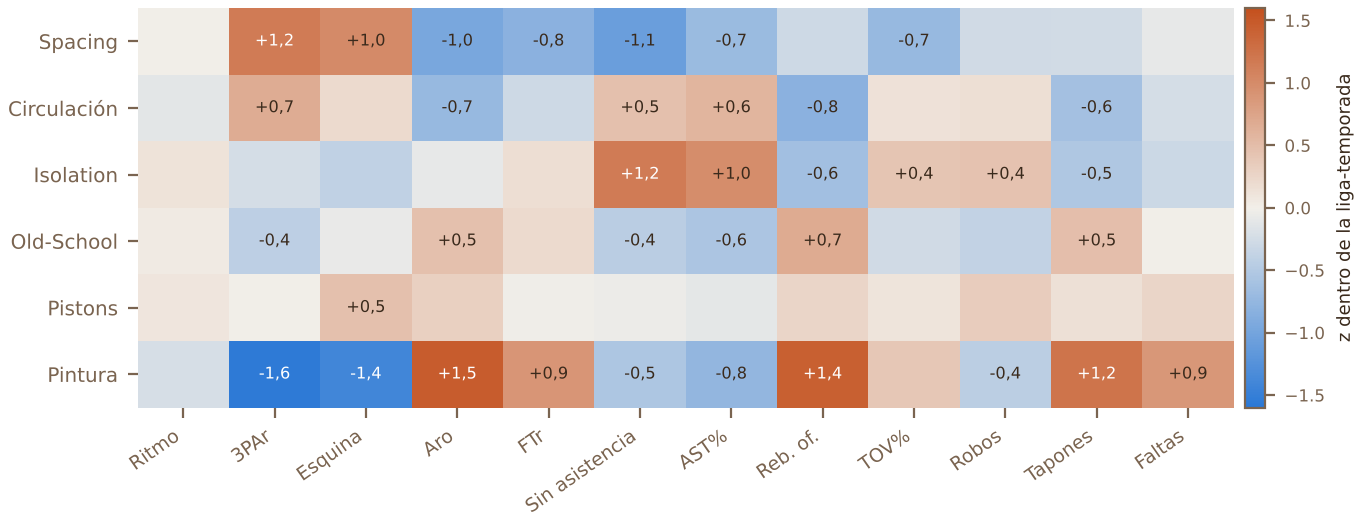
\includegraphics[width=\linewidth]{fit_v2_figuras/fig_ii_estilos.png}
\captionof{figure}{Centroides de los seis estilos unificados en los 12 rasgos (z de jugadores dentro de su liga-temporada; \texttt{estilos.json}). Escala divergente con el 0 (la media de la liga) en gris claro; se rotulan los valores con |z| \ensuremath{\geq} 0,4.}
\end{center}
Asignación [verificado]: 2.472 equipos-temporada y 31.428 jugadores-etapa (\ensuremath{\geq} 40 min); 658 tramos equipo-entrenador y 6.439 jugador-entrenador; con relevo, el estilo principal cambia en el 52 \% de los clubes. El 45 \% de los equipos y el 47 \% de los jugadores fiables son «puros»; seguridad media 0,74 (equipos) y 0,75 (jugadores). \textbf{Correspondencia con VaDE}: ARI 0,031 y NMI 0,046 en 1.667 equipos-temporada: las dos taxonomías casi no coinciden porque VaDE usa rasgos en la vara EuroLeague con el nivel neutralizado y cuotas por posición, y esta usa rangos dentro de la liga y arquetipos de jugador. \textbf{Coherencia jugador--equipo}: la mezcla de estilos de los jugadores (por minutos) acierta el estilo del equipo en el 33 \% de los casos (azar con esas frecuencias: 21 \%): el estilo del equipo describe su desviación frente a su liga, no su plantilla. Ejemplos y lectura para dirección deportiva en \texttt{docs/\allowbreak{}glosario.md}.


\section*{21. Adaptación al cambio de liga (F7)}
\addcontentsline{toc}{section}{21. Adaptación al cambio de liga (F7)}
La normalización (F2) dice qué rendimiento cabe esperar de un jugador en otra liga \textbf{si se comportara como el puente medio}. La F7 mide la parte que la normalización no explica: cuánto se desvía de lo esperado quien cambia de liga, según quién es y hacia dónde va, y cómo evoluciona partido a partido (\texttt{bbfit/\allowbreak{}adaptacion.py}, \texttt{configs/\allowbreak{}adaptacion.yaml}).

\subsection*{21.1 Traspasos y valor esperado}
Traspaso = la persona juega la liga B en $t+1$ sin haberla jugado en $t$ (origen: la de más minutos que deja, \texttt{salida}, o la de más minutos si no deja ninguna, \texttt{adicion}), o B empieza dentro de la temporada cuando A ha terminado y la pareja no es concurrente; origen con \ensuremath{\geq} 150 min. \textbf{5.040 traspasos} de 2.530 personas en 172 parejas de ligas: 3.705 salidas, 1.224 adiciones, 111 dentro de la temporada [verificado]. El valor esperado invierte la traducción amortiguada de la variante elegida hacia la escala de destino:

\[
\begin{aligned} \theta' &= \theta + \mathrm{d}(\text{edad})\cdot\text{años}, \qquad z_d = \frac{\theta' - \delta_{\mathrm{dest}}}{\lambda\,s_{\mathrm{dest}}}, \qquad \hat y = T^{-1}\!\big(\mu_{\mathrm{dest},t,\mathrm{pos}} + \tau_{\mathrm{dest},\mathrm{pos}}\, z_d\big),\\ \operatorname{Var}(\hat y) &\approx \Big(\frac{\tau}{\lambda s}\Big)^2\big(\mathrm{sd}_\theta^2 + \mathrm{sd}_\delta^2 + \eta^2\big) \quad (\text{en la escala transformada}) . \end{aligned}
\]
Comprobación: correlación 0,93-0,96 con las predicciones sin fuga de la F2 en los mismos 577 casos [verificado]. $L$ se calcula con la misma fórmula del índice de nivel sobre la capacidad esperada y la observada; $L_{\mathrm{rel}}$ es la media geométrica de $y/\hat y$ de las 8 métricas de nivel (DRtg invertido) y es el ADAPT\% principal.

\subsection*{21.2 Modelo jerárquico del desvío}
\[
\begin{aligned} \log\frac{y_i}{\hat y_i} &= \mathbf x_i^{\top}\boldsymbol\beta + u_{o(i)\to d(i)} + v_{e(d(i))} + \varepsilon_i, \qquad \varepsilon_i \sim \mathcal N\!\big(0, \sigma^2/w_i\big),\\ w_i &= \frac{\mathrm{min}_i}{\mathrm{min}_i + 600}\cdot \mathrm{IPCW}_i,\\ \boldsymbol\beta &\sim \mathcal N(\mathbf 0, \mathbf I), \quad u \sim \mathcal N(0, \tau_u^2), \quad v \sim \mathcal N(0, \tau_v^2), \quad \sigma^2, \tau_u^2, \tau_v^2 \sim \mathrm{IG}(1,\, 0{,}001) , \end{aligned}
\]
con muestreo de Gibbs propio (2 cadenas \ensuremath{\times} 3.000 iteraciones, $\hat R \le 1{,}006$) y $L$ aditivo ($\Delta L$). Covariables: grupo de nacionalidad (9 grupos: \texttt{EEUU\_a\_Europa}, \texttt{otro\_desde\_EEUU}, \texttt{hacia\_EEUU}, \texttt{intra\_EEUU}, \texttt{nacional\_mismo\_pais}, \texttt{extranjero\_mismo\_pais}, \texttt{europeo\_cambia\_liga}, \texttt{extranjero\_cambia\_pais}, \texttt{desconocido}; nacionalidad = moda de 4 fuentes, nunca imputada), posición, arquetipo F6, edad y edad\ensuremath{^{2}}, rol de origen y cambio de rol (F3), salto de nivel con signo y absoluto (F2), distancia de estilo entre equipos, cambio de entrenador, traspaso dentro de la temporada, adición y regreso; lo que falta entra como 0 con su bandera. Canterano: no hay fuente (NaN y bandera).

\subsection*{21.3 Curva temporal, censura y ADAPT\%}
\[
\begin{aligned} y_{ig} &= A_i\big(1 + D\,e^{-g/\kappa}\big), \qquad \log\kappa \sim \mathcal N(\log 5, 1), \quad D \sim \mathcal N(0,\, 0{,}15^2),\\ g_{q} &= \kappa\,\ln\frac{1}{1-q}\quad (\text{partidos hasta cerrar la fracción } q \text{ del hueco inicial}) , \end{aligned}
\]
ajustada dentro de jugador ($A_i$ libre) por máximo a posteriori con bootstrap de jugadores (200), sobre los primeros 80 partidos en la liga nueva, y \textbf{también sobre un grupo de control} (3.726 jugadores que siguen en su equipo): la curva neta divide por la del control para separar el «arranque de temporada» común a todos. \textbf{Censura}: observado = juega \ensuremath{\geq} 25 \% de los minutos de su equipo desde que llega y \ensuremath{\geq} 150 min; un logit de seguir observado con las covariables, el nivel de origen y el rendimiento de sus 5 primeros partidos da $\mathrm{IPCW}_i = 1/\hat p_i$ (recortado p2-p98); 2026-27 es censura administrativa. La interfaz para el simulador devuelve, por celda (par de ligas + grupo + posición) con reserva jerárquica celda \ensuremath{\to} par \ensuremath{\to} escalón \ensuremath{\to} global (primer nivel con $n \ge 8$), la mejor aproximación $1 + \delta e^{-g/\kappa}$ (mínimos cuadrados en 60 partidos, $\kappa \le 500$) de la trayectoria

\[
T(g) = \big(1 + \Delta_{\mathrm{temp}}\big)\,\frac{1 + D\,\varphi_g}{1 + D\,\bar w}, \qquad \mathrm{ADAPT\%}_i = 100\,\frac{\mathbb E[y_{i,\mathrm{dest}}]}{\hat y_i} = 100\,e^{\bar\eta_i} .
\]
\begin{center}
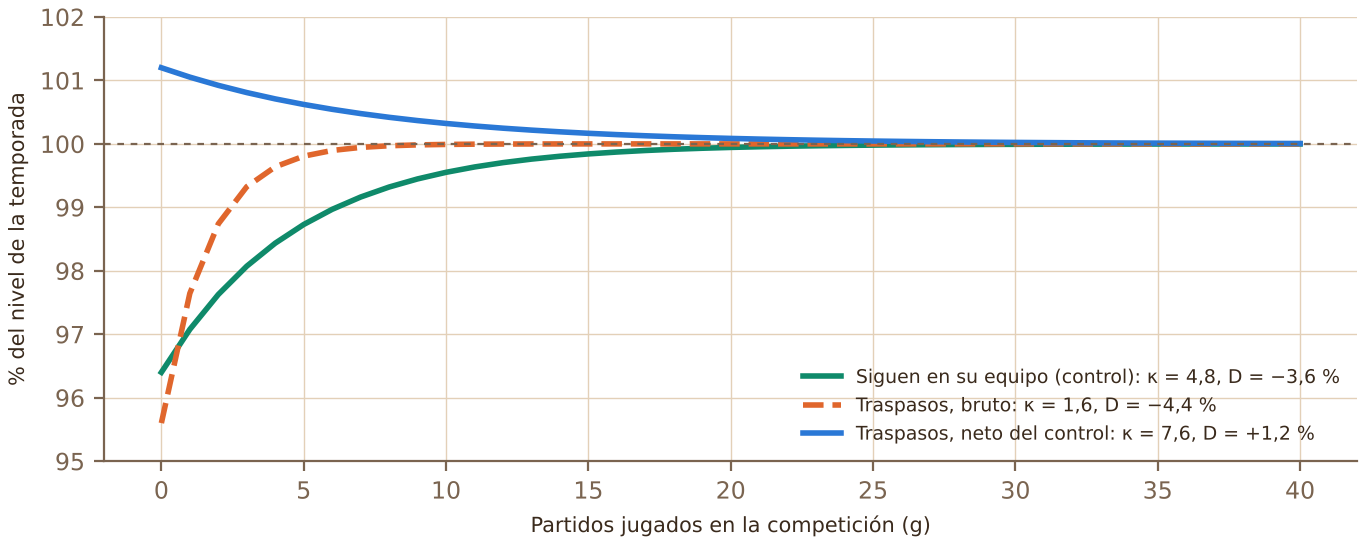
\includegraphics[width=\linewidth]{fit_v2_figuras/fig_ii_adaptacion.png}
\captionof{figure}{Curva de adaptación $1 + D e^{-g/\kappa}$ en producción por 100 posesiones con los parámetros del informe F7: todos arrancan la temporada \textasciitilde{}2-4 \% por debajo, también los que no cambian de equipo; el traspaso no muestra un hueco adicional distinguible de 0 (curva neta).}
\end{center}
\begin{center}\small
\captionof{table}{\ensuremath{\Delta} de temporada (ADAPT\% compuesto $L_{\mathrm{rel}}$, con IPCW; intervalo del 90 \%) por grupo de nacionalidad (informe F7) [estimado]. Global: +1,1 \% [+0,5, +1,7] (n = 2.491).}
\resizebox{\ifdim\width>\linewidth\linewidth\else\width\fi}{!}{%
\begin{tabular}{lrllll}
\toprule
Grupo & n & \ensuremath{\Delta} $L_{\mathrm{rel}}$ & \ensuremath{\Delta} pts/100 & \ensuremath{\Delta} TS\% & \ensuremath{\Delta} PER \\
\midrule
EEUU\_a\_Europa & 231 & \ensuremath{-}1,2 \% [\ensuremath{-}2,9, +0,6] & +2,4 \% [+0,2, +4,7] & \ensuremath{-}1,6 \% [\ensuremath{-}2,8, \ensuremath{-}0,5] & \ensuremath{-}0,5 \% [\ensuremath{-}3,2, +2,3] \\
europeo\_cambia\_liga & 364 & +2,3 \% [+0,9, +3,7] & +1,3 \% [\ensuremath{-}0,4, +3,1] & +0,9 \% [0,0, +1,9] & +1,7 \% [\ensuremath{-}0,6, +4,1] \\
extranjero\_cambia\_pais & 617 & +2,7 \% [+1,5, +3,9] & +4,4 \% [+2,9, +5,8] & +0,3 \% & +3,5 \% [+1,7, +5,3] \\
nacional\_mismo\_pais & 248 & \ensuremath{-}3,3 \% [\ensuremath{-}5,1, \ensuremath{-}1,5] & \ensuremath{-}2,5 \% [\ensuremath{-}4,7, \ensuremath{-}0,1] & \ensuremath{-}1,5 \% & \ensuremath{-}6,4 \% [\ensuremath{-}9,0, \ensuremath{-}3,7] \\
desconocido & 729 & +1,2 \% [+0,1, +2,2] & \ensuremath{-}0,1 \% & 0,0 \% & 0,0 \% \\
\bottomrule
\end{tabular}}
\end{center}
\textbf{Hipótesis del estadounidense} (no supuesta, contrastada): frente al europeo que cambia de liga, el estadounidense en su primer año europeo rinde \textbf{\ensuremath{-}6,8 \% [\ensuremath{-}9,7, \ensuremath{-}3,8]} en $L_{\mathrm{rel}}$ (P(< 0) = 1,00), \ensuremath{-}7,9 \% en PER, \ensuremath{-}4,3 \% en TS\% y en pts/100; robusto sin las covariables de rol (\ensuremath{-}5,7 \%) y sin IPCW (\ensuremath{-}5,1 \%). Adaptación más lenta: \textbf{no se detecta} (hueco medio de los partidos 1-5 +2,8 \% [\ensuremath{-}2,3, +5,8] en pts/100; ganancia de la 2.ª temporada +3,2 \% [\ensuremath{-}1,6, +7,0]). \textbf{Curva}: control \ensuremath{\kappa} = 4,8 [2,6, 17,9], D = \ensuremath{-}3,6 \%, 3,4 / 11,2 partidos al 50 / 90 \%; traspasos netos \ensuremath{\kappa} = 7,6 [1,0, 18,2], D = +1,2 \% [\ensuremath{-}5,6, +3,0]: \ensuremath{\kappa} está mal identificado cuando el hueco es \ensuremath{\approx} 0, y el efecto de temporada es persistente (\ensuremath{\kappa} de la interfaz casi siempre grande). Grupos con hueco propio: NBA \ensuremath{\leftrightarrow} G League (\ensuremath{-}13 \%, \ensuremath{\kappa} \ensuremath{\approx} 25-40) y Europa \ensuremath{\to} NBA (\ensuremath{-}5 a \ensuremath{-}7 \%). \textbf{Censura}: el 61,5 \% de 4.172 llegadas llega a ser observada; los censurados rinden peor desde el principio (log-cociente de pts/100 en sus 5 primeros partidos \ensuremath{-}0,140 frente a \ensuremath{-}0,010); el IPCW baja el \ensuremath{\Delta} medio de pts/100 de +3,5 \% a +1,5 \% y el de $L_{\mathrm{rel}}$ de +2,2 \% a +1,1 \%: sin corrección se sobreestima la adaptación en \ensuremath{\approx} 1-2 puntos [verificado + estimado].

\textbf{Examen sin fuga del ADAPT\%} (ajuste con destino \ensuremath{\leq} $t$, predicción de $t+1$; cortes 2022-2024; 1.644-1.692 casos por métrica): MAE del log-cociente en pts/100 0,177 \ensuremath{\to} 0,169 (\ensuremath{-}5,0 \%), PER \ensuremath{-}2,1 \%, AST\% \ensuremath{-}1,4 \%, USG\% \ensuremath{-}1,6 \%, TS\% +0,4 \%, $L_{\mathrm{rel}}$ \ensuremath{-}0,4 \%; cobertura del 80 \% 0,81-0,83; estricto (\ensuremath{\hat y} de la F2 también sin fuga): pts/100 \ensuremath{-}6,2 \%. Calibración: buena en muestra, pero fuera de muestra las predicciones son \textbf{demasiado extremas} (decil bajo 89 \ensuremath{\to} 93 observado, alto 113 \ensuremath{\to} 107; pendiente \ensuremath{\approx} 0,55): hay que encoger el ADAPT\% previsto hacia 100 o usar el intervalo predictivo [verificado].


\section*{22. Simulador de encaje v2 (F8)}
\addcontentsline{toc}{section}{22. Simulador de encaje v2 (F8)}
El usuario elige \textbf{sólo} jugador y club de destino (y, opcionalmente, un escenario de plantilla: quién no está). No se teclean minutos: el rol y los minutos son endógenos. Cada iteración Monte Carlo (semilla fija; 1.000 iteraciones por jugador-club, \texttt{configs/\allowbreak{}simulation.yaml}) encadena las capas de las fases 2-7 en ocho pasos (\texttt{bbfit/\allowbreak{}simulador.py}, insumos en \texttt{bbfit/\allowbreak{}sim\_insumos.py}). Esta sección describe el diseño; los resultados de la validación se completarán con el informe de la fase 8 (marcadores amarillos «F8»).

\subsection*{22.1 Flujo generativo}
\begin{enumerate}
  \item \textbf{Nivel latente traducido al destino} (F2): capacidad $\theta_m$ de cada métrica con su desviación, deriva por edad, nivel de la competición de destino con su incertidumbre acumulada y desviación de temporada $\psi$: $z_d = \big(\theta + \text{deriva} + \mathrm{sd}\,\varepsilon_1 - (\delta_d + \mathrm{sd}_\delta\,\varepsilon_2)\big)/s_d + \sqrt{\psi_d}\,\varepsilon_3$, valor $= T^{-1}(\mu_{d,\mathrm{pos}} + \tau_{d,\mathrm{pos}} z_d)$.
  \item \textbf{Adaptación} (F7): factor $a_g = 1 + \Delta\,e^{-g/\kappa}$ por partido, con $\Delta$ del prior de la celda contraído por 0,55 (la pendiente de calibración fuera de muestra); la producción de la temporada se multiplica por su media en los partidos que juega y $\mathrm{ADAPT\%} = 100\cdot\overline{a_g}$.
  \item \textbf{Rol y minutos endógenos} (F3-F4): asignación de Plackett-Luce sobre la plantilla de destino con el fichaje, utilidad $u_i = \sum_k w_k x_{ik}$ (nivel $L$, minutos previos en el club o fuera, nuevo, sin dato, encaje posicional y de estilo, edad y edad\ensuremath{^{2}}; $w$ por máxima verosimilitud de las rotaciones reales), restricciones de posición, tamaño de rotación y curva de reparto del entrenador de destino. GO-TO-GUY = TITULAR por minutos y top-2 del equipo en el GTI proyectado, $\mathrm{GTI}' = \mathrm{GTI}_0 + 2\,\big(z(\mathrm{USG}') - z(\mathrm{USG}_0)\big)$, con umbral 4,0.
  \item \textbf{Uso} (suma fija): $f = 20\sum_i m_i / \sum_i m_i\,\mathrm{USG}_i$, $\mathrm{USG}'_i = \mathrm{USG}_i\,(1 + a(f-1))$ con $a$ = 0,5; curva uso--eficiencia $\mathrm{TS}' = \mathrm{TS} + \beta\,\Delta\mathrm{USG}$, $\beta \sim \mathcal N(\beta_{\mathrm{pos3}}, \mathrm{sd})$ (IV de la F4), y $\mathrm{P100}' = \mathrm{P100}\,(\mathrm{USG}'/\mathrm{USG})(\mathrm{TS}'/\mathrm{TS})$.
  \item \textbf{Calidad de compañeros}: $\bar L$ = media de $L$ de los compañeros ponderada por sus minutos simulados; $\mathrm{TS} \mathrel{+}= b\,(\bar L - \bar L_{\mathrm{origen}})$, con $b$ muestreado de su intervalo (F4).
  \item \textbf{Estilo} (F6): divergencia de Jensen-Shannon entre el vector de estilo unificado del jugador y el del equipo, complementariedad (cubre un hueco de estilo frente a la composición típica de los equipos de ese estilo) y efecto en la entropía del reparto de uso y de la red de pases (F5). Entra en la utilidad de minutos y en el Fit.
  \item \textbf{Ruido personal}: $\sigma_i$ (F5) para pts/100 y ruido de muestreo del algoritmo A para el resto, según las posesiones simuladas.
  \item \textbf{Ritmo y competición}: por partido = por 100 \ensuremath{\times} posesiones del club de destino en sus minutos / 100.
\end{enumerate}
\[
\begin{aligned} \mathrm{JS}(\mathbf p \,\|\, \mathbf q) &= \tfrac12 \mathrm{KL}(\mathbf p \,\|\, \mathbf m) + \tfrac12 \mathrm{KL}(\mathbf q \,\|\, \mathbf m),\quad \mathbf m = \tfrac12(\mathbf p + \mathbf q) \quad (\text{bits; entre 0 y 1}),\\ \mathrm{Fit} &= b_0 + \sum_{f} w_f\,\frac{x_f - \bar x_f}{\mathrm{sd}_f} = b_0 + \sum_{C} \underbrace{\sum_{f \in C} w_f\,\frac{x_f - \bar x_f}{\mathrm{sd}_f}}_{\text{componente } C} . \end{aligned}
\]
\subsection*{22.2 Salidas e índice Fit}
Por jugador-club: reparto de roles y minutos esperados; producción por 100 y por partido con intervalos del 50 \% y del 90 \%; curva de adaptación y ADAPT\% esperado (temporada y primeros 10 partidos); impacto en el Net del equipo y quintetos más probables; índice \textbf{Fit} descompuesto de forma aditiva y exacta en seis componentes $C$: \textbf{nivel} ($L$ efectivo menos el de los compañeros), \textbf{rol} (índice de rol esperado), \textbf{estilo} (\ensuremath{-}JS), \textbf{complementariedad} (hueco de estilo y cambio de entropía de uso y de pases), \textbf{adaptación} (ADAPT\% \ensuremath{-} 100) y \textbf{riesgo} (volatilidad relativa a la liga, incertidumbre del nivel, $H^{\mathrm{rol}}$). Los pesos $w_f$ salen de una regresión ridge (penalización 1) del éxito real, $0{,}5\,z(\mathrm{MIN\%}) + 0{,}5\,z(\mathrm{pts}/100)$ dentro de la liga-temporada de destino, ajustada sólo con cortes anteriores; la unidad del Fit es la DT de ese éxito. \textbf{Avisos} automáticos: muestra pequeña (< 300' o < 10 partidos), salto de nivel grande (> 0,6 DT), incertidumbre alta (sd > 0,45 DT), cambio de rol de \ensuremath{\geq} 2 escalones, volatilidad por encima del percentil 80 de la liga y adaptación estimada con poca información propia (reserva global o $n$ < 8).

\subsection*{22.3 Protocolo de validación}
\begin{itemize}
  \item \textbf{Examen temporal sin fuga}: para cada fichaje real $t \to t+1$ (persona con registro en $t$ que en $t+1$ juega en un club en el que no estaba) se simula con insumos de $t$ y modelos ajustados con \ensuremath{\leq} $t$; cortes 2021-22 a 2024-25, y 2023-24 y 2024-25 con la normalización también reajustada con \ensuremath{\leq} $t$.
  \item \textbf{Escenario de plantilla} = lo que sabría un director deportivo al fichar: los compañeros del club de destino que ya jugaban al empezar la temporada (primer partido en el primer 20 \% del calendario); nada de su rendimiento en $t+1$. Variante «real»: todos los que pasaron por la plantilla, con su presencia.
  \item \textbf{Métricas}: MAE de minutos por partido jugado; acierto de rol, matriz de confusión y log-loss multiclase; RMSE y MAE de la producción por 100 en unidades de la liga de destino (\ensuremath{\geq} 300 min en destino); cobertura de los intervalos del 50 \% y del 90 \%; desglose por liga de origen, grupo de nacionalidad, posición, rol y distancia de nivel; dejando fuera una liga.
  \item \textbf{Modelos de referencia}: (a) la lógica del simulador anterior del Atlas (producción normalizada + proyección de contexto, minutos = los de origen) y (b) un modelo simple (producción normalizada + rol de origen); diferencias con intervalos bootstrap pareados por fichaje (2.000 remuestreos, IC 90 \%).
  \item \textbf{Calibración y pesos sin fuga}: temperatura de Plackett-Luce (rejilla 0,6-1,3) y jugadores extra en la rotación (0, 2, 4) calibrados con 600 fichajes del corte anterior; pesos de la utilidad y del Fit en orden cronológico (el corte $t$ usa sólo cortes < $t$).
\end{itemize}
\subsection*{22.4 Resultados}
\fochopendiente{número de fichajes evaluados por corte y cobertura de insumos}

\begin{center}\small
\captionof{table}{Validación del simulador frente a los modelos de referencia (examen temporal sin fuga).}
\resizebox{\ifdim\width>\linewidth\linewidth\else\width\fi}{!}{%
\begin{tabular}{lllll}
\toprule
Métrica & Simulador v2 & Ref. (a) Atlas anterior & Ref. (b) simple & Diferencia (IC 90 \%) \\
\midrule
MAE minutos por partido & \fochopendiente{MAE minutos} & \fochopendiente{MAE minutos (a)} & \fochopendiente{MAE minutos (b)} & \fochopendiente{diferencia minutos} \\
Acierto de rol / log-loss & \fochopendiente{acierto de rol y log-loss} & \fochopendiente{rol (a)} & \fochopendiente{rol (b)} & \fochopendiente{diferencia rol} \\
RMSE pts/100 & \fochopendiente{RMSE producción} & \fochopendiente{RMSE (a)} & \fochopendiente{RMSE (b)} & \fochopendiente{diferencia producción} \\
Cobertura 50 \% / 90 \% & \fochopendiente{cobertura de los intervalos} & -- & -- & -- \\
\bottomrule
\end{tabular}}
\end{center}
\fochopendiente{pesos aprendidos de la utilidad de Plackett-Luce y del índice Fit} \fochopendiente{resultados dejando fuera una liga y por grupo de nacionalidad} \fochopendiente{ejemplo de simulación de un fichaje real con su Fit descompuesto}

\textbf{Límites conocidos de antemano}: el simulador hereda las incertidumbres de sus piezas (\ensuremath{\beta} uso--eficiencia con intervalo que incluye el 0; ADAPT\% demasiado extremo fuera de muestra, de ahí la contracción 0,55; estilo de equipo poco estable, ARI 0,52; un entrenador por temporada en las FEB). \fochopendiente{limitaciones y riesgos medidos en la validación}


\section*{23. Supuestos, validación y limitaciones de la Parte II}
\addcontentsline{toc}{section}{23. Supuestos, validación y limitaciones de la Parte II}
\begin{center}\small
\captionof{table}{Resumen por fase: supuesto principal, cómo se validó y limitación más relevante (cifras de los informes de fase).}
\resizebox{\ifdim\width>\linewidth\linewidth\else\width\fi}{!}{%
\begin{tabular}{llll}
\toprule
Fase & Supuesto principal & Validación & Limitación \\
\midrule
F1 FEB & El token anónimo de la página pública y la API seguirán disponibles [supuesto] & Contrato de datos: 100 \% en tipos, identidades y marcador; minutos \ensuremath{\geq} 99 \% & Jugada a jugada en texto (2022-24) sin coordenadas y con rebotes omitidos; un entrenador por temporada \\
F2 Nivel & Selección de los puentes sólo por lo observable (IPW) & Examen temporal con dos cortes (MAE 1,006 / 1,000; cobertura 0,829 \ensuremath{\to} 0,841); dejar fuera una liga & No mejora la predicción puntual; peor en pts/100, USG\% y PER entre Segunda y Tercera FEB \\
F3 Roles & USG de tiro ordena igual que el USG con pérdidas [supuesto] & 93 \% de los máximos anotadores GO-TO-GUY o TITULAR; casos conocidos & Umbral del GTI elegido (\ensuremath{\approx} 1 GO-TO-GUY por equipo); G League con entrenador sólo en el 48-96 \% de partidos \\
F4 Reemplazo & Exclusión del instrumento: la ausencia afecta al TS\% sólo vía el uso [supuesto] & Identidad contable exacta ($10^{-13}$); IC bootstrap de personas & \ensuremath{\beta} no distinguible de 0; asociaciones con \ensuremath{\Delta} Net no causales \\
F5 Entropía & Prior de liga Dirichlet (\ensuremath{\alpha} = 5) & Tests sintéticos; intervalos por muestreo & $\sigma_i$ mezcla volatilidad y ruido no modelado; NBA con una categoría menos \\
F6 Estilos & Arquetipos de jugador describen también a los equipos (desviación frente a su liga) & BIC + ARI bootstrap; firmas por método húngaro & K en el filo (5-7); estilo de equipo poco estable (ARI 0,52); coherencia jugador-equipo 33 \% \\
F7 Adaptación & Censura informativa corregible por IPCW con lo observable & Examen temporal 2022-2024, dejar fuera una liga, calibración & Predicciones demasiado extremas fuera de muestra (pendiente \ensuremath{\approx} 0,55); 29 \% de nacionalidades desconocidas \\
F8 Simulador & Las capas se combinan de forma multiplicativa/aditiva sin interacciones no modeladas [supuesto] & Examen temporal sin fuga frente a dos referencias, bootstrap pareado & \fochopendiente{limitación principal medida} \\
\bottomrule
\end{tabular}}
\end{center}

\section*{24. Reproducibilidad de la Parte II}
\addcontentsline{toc}{section}{24. Reproducibilidad de la Parte II}
Cada paso lee las salidas del anterior; los modelos registran su ejecución (parámetros, semilla, métricas y artefactos) en MLflow, almacén local \texttt{experimentos/\allowbreak{}mlruns} (no versionado). Orden:

\begin{enumerate}
  \item Datos FEB: \texttt{python -m bbstats historico --ligas feb1 feb2 feb3} (descarga; sin red: \texttt{--sin-descarga}), \texttt{python -m bbstats feb} (partidos con grupo, cobertura, posesiones, sesgo de registro), \texttt{python -m bbstats contrato --ligas feb1 feb2 feb3}, \texttt{python -m bbstats entrenadores --ligas feb1 feb2 feb3 --sin-descarga} y \texttt{python -m bbmodel crosswalk}.
  \item Normalización: \texttt{python -m bbmodel pista}, \texttt{python -m bbmodel ajustar} y \texttt{python -m bbmodel ajustar-b}, \texttt{python -m bbmodel amortiguar} (examen: \texttt{--validar --variante V} y \texttt{--elegir}), \texttt{python -m bbmodel dataset-normalizado}, \texttt{python -m bbmodel contexto}, de nuevo \texttt{dataset-normalizado}, \texttt{python -m bbmodel interacciones} y \texttt{python -m bbmodel escalas}.
  \item Encaje v2: \texttt{python -m bbfit roles}, \texttt{python -m bbfit reemplazo}, \texttt{python -m bbfit entropia}, \texttt{python -m bbfit estilos}, \texttt{python -m bbfit adaptacion} y el simulador (\texttt{python -m bbfit simular --jugador \ldots{} --club \ldots{}}). \fochopendiente{órdenes del simulador (pesos, examen temporal, histórico, exportación) en su orden de ejecución}
  \item Este documento: \texttt{python -m bbestilo articulo} (equivalente: \texttt{python -m bbfit.articulo}), que escribe el PDF, su copia en \texttt{artifact/\allowbreak{}articulo/\allowbreak{}} y el LaTeX autónomo \texttt{docs/\allowbreak{}articulo/\allowbreak{}fit\_v2.tex}.
  \item Pruebas: \texttt{python -m pytest -q}.
\end{enumerate}
Los umbrales e hiperparámetros están en \texttt{configs/\allowbreak{}*.yaml} (\texttt{normalization}, \texttt{roles}, \texttt{reemplazo}, \texttt{entropia}, \texttt{styles}, \texttt{adaptacion}, \texttt{simulation}); el diccionario de datos en \texttt{docs/\allowbreak{}data\_dictionary.md} y el glosario para dirección deportiva en \texttt{docs/\allowbreak{}glosario.md}.

\section*{Referencias}
\begin{enumerate}[label={[\arabic*]}]
  \item Adams, R. P. y MacKay, D. J. C. (2007). Bayesian online changepoint detection. arXiv:0710.3742.
  \item Angrist, J. D. e Imbens, G. W. (1995). Two-stage least squares estimation of average causal effects in models with variable treatment intensity. Journal of the American Statistical Association, 90(430), 431-442.
  \item Barlow, R. E., Bartholomew, D. J., Bremner, J. M. y Brunk, H. D. (1972). Statistical Inference under Order Restrictions. Wiley.
  \item Efron, B. y Morris, C. (1975). Data analysis using Stein's estimator and its generalizations. Journal of the American Statistical Association, 70(350), 311-319.
  \item Fritsch, F. N. y Carlson, R. E. (1980). Monotone piecewise cubic interpolation. SIAM Journal on Numerical Analysis, 17(2), 238-246.
  \item Gelman, A., Carlin, J. B., Stern, H. S., Dunson, D. B., Vehtari, A. y Rubin, D. B. (2013). Bayesian Data Analysis (3.ª ed.). CRC Press.
  \item Horvitz, D. G. y Thompson, D. J. (1952). A generalization of sampling without replacement from a finite universe. Journal of the American Statistical Association, 47(260), 663-685.
  \item Kuhn, H. W. (1955). The Hungarian method for the assignment problem. Naval Research Logistics Quarterly, 2, 83-97.
  \item Lin, J. (1991). Divergence measures based on the Shannon entropy. IEEE Transactions on Information Theory, 37(1), 145-151.
  \item Luce, R. D. (1959). Individual Choice Behavior: A Theoretical Analysis. Wiley.
  \item Plackett, R. L. (1975). The analysis of permutations. Journal of the Royal Statistical Society C, 24(2), 193-202.
  \item Robins, J. M. y Finkelstein, D. M. (2000). Correcting for noncompliance and dependent censoring in an AIDS clinical trial with inverse probability of censoring weighted (IPCW) log-rank tests. Biometrics, 56(3), 779-788.
  \item Shannon, C. E. (1948). A mathematical theory of communication. Bell System Technical Journal, 27, 379-423.
  \item Saski Baskonia, Dirección Deportiva (2026). Informes de fase del encaje v2 (\texttt{docs/\allowbreak{}checkpoints/\allowbreak{}F1.md} \ldots{} \texttt{F8.md}), normalización amortiguada (\texttt{docs/\allowbreak{}normalizacion\_amortiguada.md}), diccionario de datos y glosario. Documentación interna.
\end{enumerate}
\end{document}
